\chapter{Experimentos Númericos}
\section{Método Numérico }
 
\begin{example}
Vamos a tomar la siguiente ecuación diferencial 
\begin{equation}
	\left\lbrace \begin{array}{l}
		d(u')=-u' d\delta_{\hat{t}}\\
		u(0)=0\\
		u'(0)=1
	\end{array}\right. \label{eq:3.1}
\end{equation} 
Donde $d\delta_{\hat{t}}(A)=\left\lbrace \begin{array}{l}
	0 \; si \; \hat{t}\notin A\\
	1 \; si \; \hat{t}\in A
\end{array}\right. $

Una solución de \ref{eq:3.1}   es una función de variación acotada y continua a izquierda $u'$ tal que  para cualquier conjunto $A$ de Borel
\begin{equation*}
	\mu_{u'}(A)=\int_A-u'(s)\: d\delta_{\hat{t}}(s)
\end{equation*}
donde $\mu_{u'}$ es la medida generada por $u'$. Si tomamos el intervalo $[0,t)$ entonces 
$$u'(t)-u'(0)=\mu_{u'}([0,t))=\int_{[0,t)}-u'(s)\: d\delta_{\hat{t}}(s)$$
 Podemos trasformar esta ecuación \ref{eq:3.1} en un sistema de ecuaciones de la siguiente manera
 \begin{multicols}{2}

 	$\left\lbrace \begin{array}{l}
 		d(u)=vd\lambda\\
 		d(v)=-v d\delta_{\hat{t}}\\
 		u(0)=0\\
 		v(0)=1
 	\end{array}\right. $
 
 	$\left\lbrace \begin{array}{l}
 		u(t)=\displaystyle\int_{0}^{t}v(s) \; ds\\
 		\\
 		v(t)=1-\displaystyle\int_{[0,t)}v(s) \; d\delta_{\hat{t}}(s)
 	\end{array}\right. $
 
\end{multicols}
%cuya solución es
%
%
%\begin{multicols}{2}
%$v(t)=\left\lbrace \begin{array}{l}
%			1 \; si \; t\leq \hat{t}\\
%			0 \; si \; t> \hat{t}
%		\end{array}\right. $
%				 
%			$u(t)=\left\lbrace \begin{array}{l}
%				t \; si \; t\leq \hat{t}\\
%				\hat{t} \; si \; t> \hat{t}
%			\end{array}\right. $
%\end{multicols}
%
%
%


Si tomamos la partición del intervalo $[0,T]$, 
$$P_N=\{0=t_0,t_1, t_2,\cdots,t_n\cdots, t_N=T\}$$
podemos aproximar $$\displaystyle\int_{[0,t_n)}v(s) \; d\delta_{\hat{t}}(s) \approx \sum_{j=1}^{n-1}v(t_j)\delta_{\hat{t}}\left( [t_j,t_{j+1})\right), $$ donde $\{t_0=0,t_1,\cdots , t_n\}\subset P_N$. Entonces 
	\begin{equation*}
		v(t_n)=v(t_0)-\sum_{j=1}^{n-1}v(t_j)\delta_{\hat{t}}\left( [t_j,t_{j+1})\right) 
	\end{equation*}
si desarrollamos tenemos que
$$\begin{array}{l}
	v(t_1)=v(t_0)\\
	v(t_2)=v(t_0)-v(t_1)\delta_{\hat{t}}([t_1,t_2))=v(t_1)-v(t_1)\delta_{\hat{t}}([t_1,t_2))\\
	v(t_3)=v(t_0)-v(t_1)\delta_{\hat{t}}([t_1,t_2))-v(t_2)\delta_{\hat{t}}([t_2,t_3))=v(t_2)-v(t_2)\delta_{\hat{t}}([t_2,t_3))\\
	\cdots\\
	v(t_n)=v(t_{n-1})-v(t_{n-1})\delta_{\hat{t}}([t_{n-1},t_n))
\end{array}$$
Como vamos a poder encontrar un $1<r<N$ tal que $\hat{t}\in [t_r,t_{r+1})$. Entonces
\begin{itemize}
	\item  $v(t_i)=1$ para $i=1\cdots r$, pues $\delta_{\hat{t}}\left( [t_i,t_{i+1})\right)=0$
	\item$v(t_{r+1})=1-v(t_{r})\delta_{\hat{t}}\left( [t_{r},t_{r+1})\right)=1-\delta_{\hat{t}}\left( [t_{r},t_{r+1})\right)=0$
	\item $v(t_i)=0$ para $i=r+1, \cdots ,N$
\end{itemize}


Luego para la partición $P_N$ tenemos que
	 \begin{equation*}
		v(t_n)=\left\lbrace \begin{array}{l}
			1 \; si \; t_n\leq \hat{t}\\
			0 \; si \; t_n> \hat{t}
		\end{array}\right. 
	\end{equation*} 
Ya teniendo $v$ puedo resolver $u$ integrando con respecto a la integral de Lebesgue:
	 \begin{equation*}
	u(t_n)=\left\lbrace \begin{array}{l}
		t _n\; si \; t\leq \hat{t}\\
		\hat{t} \; si \; t_n> \hat{t}
	\end{array}\right. 
\end{equation*} 
Entonces si agrandamos la partición del intervalo $[0,T]$ tenemos 
\begin{center}
		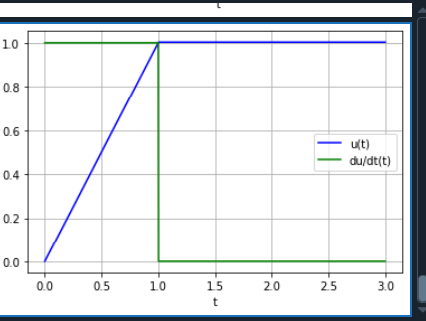
\includegraphics[width=0.7\linewidth]{fig3}
\end{center}
\vspace{0.2cm}
	
 Si aproximamos $\displaystyle\int_{[0,t_n)}v(s) \; d\delta_{\hat{t}}(s) \approx \sum_{j=1}^{n-1}\left( \dfrac{v(t_{j+1})+v(t_j)}{2}\right) \delta_{\hat{t}}\left( [t_j,t_{j+1})\right) $, donde $\{0=t_0,t_1,\cdots , t_n\}\subset P_N$. Entonces 
\begin{equation*}
	v(t_n)=v(t_0)-\sum_{j=1}^{n-1}\left( \dfrac{v(t_{j+1})+v(t_j)}{2}\right) \delta_{\hat{t}}\left( [t_j,t_{j+1})\right)
\end{equation*}
si desarrollamos tenemos que
$$\begin{array}{l}
	v(t_1)=v(t_0)\\
	v(t_2)=v(t_0)-\left[ \dfrac{v(2)+v(1)}{2}\right] \delta_{\hat{t}}([t_1,t_2))=v(t_1)-\left[ \dfrac{v(2)+v(1)}{2}\right] \delta_{\hat{t}}([t_1,t_2))\\
	v(t_3)=v(t_0)-\left[ \dfrac{v(2)+v(1)}{2}\right]\delta_{\hat{t}}([t_1,t_2))-\left[ \dfrac{v(3)+v(2)}{2}\right]\delta_{\hat{t}}([t_2,t_3))\\
	v(t_3)=v(t_2)-\left[ \dfrac{v(3)+v(2)}{2}\right]\delta_{\hat{t}}([t_2,t_3))\\
	\cdots\\
	v(t_n)=v(t_{n-1})-\left[ \dfrac{v(n)+v(n-1)}{2}\right] \delta_{\hat{t}}([t_{n-1},t_{n}))
\end{array}$$

Como vamos a poder encontrar un $1<r<N$ tal que $\hat{t}\in [t_r,t_{r+1})$. Entonces
\begin{itemize}
	\item  $v(t_i)=1$ para $i=1\cdots r$, pues $\delta_{\hat{t}}\left( [t_i,t_{i+1})\right)=0$
	\item $v(t_{r+1})=1-\dfrac{v(t_{r+1})}{2}$ luego $v(t_{r+1})=3/2$
	
	\item$v(t_{r+2})=3/2-\left[ \dfrac{v(r+2)+3/2}{2}\right]\delta_{\hat{t}}\left( [t_{r+1},t_{r+2})\right)=3/2$
	\item $v(t_i)=3/2$ para $i=r+1, \cdots ,N$
\end{itemize}
Entonces


\begin{equation*}
	v(t_n)=\left\lbrace \begin{array}{lcr}
		1 & si & t_n\leq \hat{t}\\
		2/3 & si & t_n> \hat{t}
	\end{array}\right. 
\end{equation*} 
Ya teniendo $v$ puedo resolver $u$ integrando con respecto a la integral de Lebesgue:
\begin{equation*}
	u(t_n)=\left\lbrace \begin{array}{lcr}
		t_n & si & t_n\leq \hat{t}\\
		\dfrac{2t_n+\hat{t}}{3} & si & t_n> \hat{t}
	\end{array}\right. 
\end{equation*} 
Entonces si agrandamos la partición del intervalo $[0,T]$ tenemos 
\begin{center}
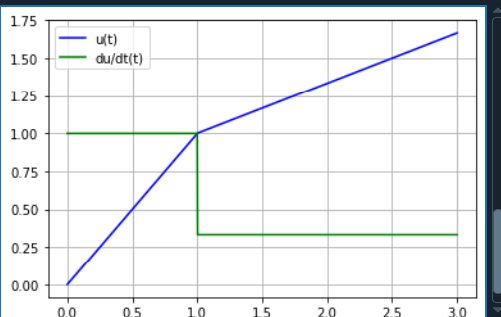
\includegraphics[width=0.7\linewidth]{fig4}
\end{center}
\end{example}
 
 
 \subsubsection{Método de Euler}
 Partimos del problema
 \begin{equation}
 	\left\lbrace \begin{array}{l} 
 			d(v)=f(t,v) d\mu\\
 			v(0)=v_0
 			\end{array}\right. \label{eq:3.2}
 \end{equation} 
 donde $f$ es una función Lipschitz en la variable vectorial, ademas $||f(t,v)||\leq \beta(t)\alpha(v)$. Una solución del problema \ref{eq:3.2} es una función continua izquierda y de variación acotada $v$ tal que
 \begin{equation}
 	v(t)=v(0)+\int_{[0,t)}f(s,v(s))\: d\mu(s) \label{eq:3.3}
 \end{equation}
 
 Queremos encontrar un algoritmo numérico para llar la solución de \ref{eq:3.2}, para ello necesitamos particionar el intervalo $[0,T]$, en $n+1$ puntos igualmente espaciados. Tenemos la partición $P_N=\{0=t_0,\cdots,t_N=T\}$  y partimos de suponer que 
 $$\int_{[t_i,t_{i+1})}f(s,v(s))\:d\mu(s)\approx f(t_i,v(t_i))\mu([t_i,t_{i+1}))$$
 
 Si llamamos $v_{i}$ a la aproximación de $v(t_i)$ mediante la suposición anterior  y  \ref{eq:3.3}, entonces 
 

 $$v_{i}=v_{i-1}+f(t_{i-1})\mu([t_{i-1},t_{i}))$$

\begin{obs}
	Sea $\mu$ es una medida de Borel, continua y finita. Si $\mu([0,T])<\infty$ entonces para la partición $P_N$ tenemos que $\exists R>0$ tal que $$\mu([t_{i-1},t_1))\leq \dfrac{R}{N}$$
\end{obs}
\begin{obs}
	Sea $v$ una función de variación acotada, entonces para la partición $P_N$  $\exists V>0$ tal que
	$$\V(v,[t_{i-1},t_i))\leq \dfrac{V}{N}$$ 
\end{obs}
\textbf{Veamos que error cometemos con este método.}
Si dividimos la medida $\mu$ en suma de una medida continua $\bar{\mu}$ y una discontinua $\mu_a$ según la definición \ref{mu_a}.
\begin{itemize}
	\item  Si consideramos la ecuación \ref{eq:3.2} donde $\mu$ es una medida continua entonces el error del método de Euler es el siguiente:


 Partiendo de que $v(0)=v_0$, para el valor $t_1$ se comete el siguiente error :
\begin{multline*}
	|v(t_1)-v_1|=\left| v(0)+\int_{[0,t_1)}f(s,v(s))\; d\mu(s)-v(0)-f(0,v(0))\mu([0,t_1))\right| \\
	\leq \int_{[0,t_1)}|f(s,v(s))-f(0,v(0))|\; d\mu(s)\leq L\int_{[0,t_1)}|v(s)-v(0)|\; d\mu(s)\\
	\leq L \V(v,[0,t_1))\mu([0,t_1))
\end{multline*}
 Por las observaciones  tenemos que 
 \begin{equation}
 	|v(t_1)-v_1|\leq L \V(v,[0,t_1))\mu([0,t_1))\leq L\dfrac{VR}{N^2}
 \end{equation}
 Para $t_2$ el error sera
\begin{multline*}
	|v(t_2)-v_2|=\left| v(0)+\int_{[0,t_2)}f(s,v(s))\; d\mu(s)-v_1-f(t_1,v_1)\mu([t_1,t_2))\right| \\
	=\left| v(0)+\int_{[0,t_1)}f(s,v(s))\; d\mu(s)+\int_{[t_1,t_2)}f(s,v(s))\; d\mu(s)-v_1-f(t_1,v_1)\mu([t_1,t_2))\right| 
\end{multline*}

\begin{multline*}
	|v(t_2)-v_2|	\leq |v(t_1)-v_1|+\left|\int_{[t_1,t_2)}f(s,v(s))\; d\mu(s)-f(t_1,v_1)\mu([t_1,t_2))\right| \\
	\leq |v(t_1)-v_1|+L \int_{[t_1,t_2)}|v(s)-v_1|\; d\mu(s)\\
		\leq |v(t_1)-v_1|+L \int_{[t_1,t_2)}|v(s)-v(t_1)+v(t_1)-v_1|\; d\mu(s)\\
			\leq |v(t_1)-v_1|+L \int_{[t_1,t_2)}|v(s)-v(t_1)|\; d\mu(s)+L\int_{[t_1,t_2)}|v(t_1)-v_1|\; d\mu(s)\\
			\leq |v(t_1)-v_1|+L \int_{[t_1,t_2)}|v(s)-v(t_1)|\; d\mu(s)+L|v(t_1)-v_1|\mu([t_1,t_2))\\
			\leq (1+L\dfrac{R}{N})|v(t_1)-v_1|+\int_{[t_1,t_2)}|v(s)-v(t_1)|\; d\mu(s)\\
	\leq (1+L\dfrac{R}{N})|v(t_1)-v_1|+L\dfrac{VR}{N^2}
\end{multline*}
 Por lo tanto podemos concluir que el error en el paso $i$-ésimo es 
\begin{equation}
		|v(t_{i})-v_i|\leq(1+L\dfrac{R}{N})|v(t_{i-1})-v_{i-1}|+L\dfrac{VR}{N^2}
\end{equation}
si reemplazo el error de las aproximaciones anteriores tengo

\begin{multline*}
	|v(t_{i})-v_i|\leq\left( 1+L\dfrac{R}{N}\right) ^{i-1}|v(t_{0})-v_{0}|+\left[ 1+\left( 1+\dfrac{R}{N}\right) +\cdots+\left( 1+\dfrac{R}{N}\right) ^{i-1}\right] \dfrac{LVR}{N^2}\\
	\leq\left( 1+L\dfrac{R}{N}\right) ^{i-1}|v(t_{0})-v_{0}|+\left[ \dfrac{1-\left( 1+\dfrac{R}{N}\right)^{i-1} }{1-\left(1+\dfrac{R}{N} \right) }\right] \dfrac{LVR}{N^2}\\
	\leq\left( 1+L\dfrac{R}{N}\right) ^{i-1}\left[ |v(t_{0})-v_{0}|+\dfrac{V}{N}\right] 
\end{multline*}
Si tenemos en cuenta que $|v(0)-v_0|=0$ y que $0\leq (1+x)^n\leq e^nx$ entonces
\begin{equation}
	|v(t_i)-v_i|\leq e^{-\frac{(i-1)R}{N}}\dfrac{V}{N}
\end{equation}
Por lo tanto el error global del método de Euler tiende a $0$ cuando $N$ tiende a infinito.


\item Si consideramos al problema \ref{eq:3.2} pero ahora para la medida $\mu_a$, definida en \ref{mu_a}.
\begin{obs}
	Si $\mu$ es una medida de Borel positiva y finita y $D=\{\tau\in [0,T]/ \mu(\{\tau\})>0\}$ vale que
	$$\mu_a([0,T])=\sum_{D}\mu(\{\tau\})\leq \mu([0,T])$$
	 Entonces para la partición $P_N$  existe $R=\displaystyle\max_{1\leq i\leq N}\{\mu_a([t_{i-1},t_i])\}$ tal que
	 $$\mu_a([t_{i-1},t_))\leq \dfrac{R}{N}$$
	 
	
	
\end{obs}





\end{itemize}